\documentclass[12pt,a4paper,oneside]{report}
\usepackage[a4paper,margin=2.6cm]{geometry}
\usepackage[T1]{fontenc}
\usepackage[utf8]{inputenc}
\usepackage{lmodern}
\usepackage{microtype}
\usepackage{setspace}
\onehalfspacing
\usepackage{graphicx,booktabs,array,longtable}
\usepackage{amsmath,amssymb}
\usepackage{float}
\usepackage{hyperref}
\usepackage{natbib}
\usepackage{xcolor}
\usepackage{fancyhdr}
\setlength{\headheight}{15pt}
\usepackage{caption}
\hypersetup{colorlinks=true,urlcolor=blue!50!black,linkcolor=blue!40!black,citecolor=blue!40!black}
\setlength{\parskip}{0.35em}
\setlength{\parindent}{0pt}
\pagestyle{fancy}
\fancyhf{}
\fancyhead[L]{SACAQM capstone report -- working draft}
\fancyhead[R]{\thepage}
\renewcommand{\headrulewidth}{0.35pt}
\newcommand{\todo}[1]{\par\noindent\fcolorbox{orange!60!black}{orange!10}{\parbox{0.94\linewidth}{\textbf{WP02 update required:} #1}}\par}
\newcommand{\pmf}{PM$_{2.5}$}
\begin{document}
\begin{titlepage}
\centering
\vspace*{2cm}
{\large University of the Witwatersrand\\School of Computer Science and Applied Mathematics\par}
\vspace{2.3cm}
{\Huge\bfseries Machine Learning for Retrospective Validation of PM$_{2.5}$ Spike Events in the SACAQM Air-Quality Sensor Network\par}
\vspace{1cm}
{\large MSc Artificial Intelligence -- Capstone Project Report\par}
\vspace{1cm}
{\large \textbf{Author:} [Confirm student name and student number]\\\textbf{Supervisor:} [Confirm supervisor details]\par}
\vfill
{\large Draft prepared 19 November 2026\par}
\vspace{0.5cm}
\fcolorbox{red!60!black}{red!6}{\parbox{0.82\textwidth}{\centering\textbf{Working draft -- NOT submission ready.}\\ Corrected WP02 results, university AI declaration, student details, and final author review must be inserted.}}
\vfill
\end{titlepage}
\pagenumbering{roman}
\chapter*{AI declaration -- required front matter}
\addcontentsline{toc}{chapter}{AI declaration}
\textbf{ACTION REQUIRED BEFORE SUBMISSION.} Insert the completed, official Wits postgraduate student AI declaration form here, according to the course instructions. The Moodle download currently requires authentication and the official form has \emph{not} been reproduced or completed in this draft. Disclose accurately the assistance used in research, coding, outlining, literature assistance, report drafting and editing as the official form requires. Do not submit this placeholder in place of the official declaration.
\chapter*{Abstract}
\addcontentsline{toc}{chapter}{Abstract}
Affordable environmental sensing networks offer increased spatial coverage for air-quality monitoring, but their readings may include short-lived artefacts, sensor-specific disturbances and highly localised pollution events that are difficult to distinguish. This capstone project investigates whether supervised machine learning can assist retrospective validation of candidate fine-particulate (\pmf) spikes in the South African Consortium of Air Quality Monitoring (SACAQM) AI\_r network. The implemented pipeline identifies unusually large hourly rises, assigns provisional real or fake labels using temporal and nearby-sensor evidence, and trains a Logistic Regression classifier on selected candidate observations. A historical reproducibility audit recovered 2,040 candidate-hour rows, including 730 strictly rule-labelled rows from 677 sensor-specific events. The original chronological Logistic Regression baseline achieved rule-real precision of 0.839, recall of 0.525 and F1 of 0.646, but auditing revealed limitations in the original evaluation boundaries, event-level information timing and label independence. Accordingly, these are \emph{historical heuristic-label results}, not validated pollution-detection accuracy. The final contribution is intended to combine a corrected evaluation protocol, transparent label definitions and a controlled comparison of temporal and spatial evidence. \textbf{This abstract must be revised after WP02 and final model experiments.}
\tableofcontents
\listoffigures
\listoftables
\clearpage\pagenumbering{arabic}

\chapter{Introduction}
\section{Context and motivation}
Fine particulate pollution creates an important measurement and interpretation challenge. Particles described as \pmf{} have an aerodynamic diameter of 2.5 micrometres or smaller. Their concentrations vary over time and across neighbourhoods because emissions, atmospheric mixing, transport and meteorological conditions are not uniform. The World Health Organization (WHO) publishes health-based guideline levels for exposure to fine particles and other pollutants, including an annual \pmf{} guideline of 5~$\mu$g/m$^3$ and a 24-hour guideline of 15~$\mu$g/m$^3$ \citep{who2021}. These levels provide public-health context, but they are not the thresholds used by the candidate detection algorithm in this project. The algorithm searches for abrupt departures from each sensor's own recent behaviour rather than testing the WHO guideline.

A regional monitoring system faces a tension between measurement quality and coverage. Research-grade instruments can offer a carefully controlled reference, but their expense and maintenance requirements constrain how densely they can be deployed. Lower-cost sensing technology makes a more distributed network feasible and supports localised observation where a sparse network might miss variation. However, increasing the number of deployed devices does not eliminate sensor measurement errors or uncertainty. More coverage can also mean more opportunities for unusual, inconsistent or faulty measurements to enter an automated decision system. The question is therefore not merely whether a sensor can record a high value; it is whether that high value should be treated as evidence of a credible event.

The South African Consortium of Air Quality Monitoring (SACAQM) develops the AI\_r air-quality monitoring system as a cost-effective approach for environments where accessible environmental measurements are needed \citep{mckenzie2024}. Networked instruments can generate high-frequency measurements of particulate matter and related quantities. Such information offers opportunities for analysis that go beyond a single monitoring station: a suspicious increase at one station may be examined against its recent history and measurements from other stations. The same distributed nature that creates this opportunity also complicates the analysis, because sensors differ in sampling completeness, local surroundings and spatial separation.

A straightforward alerting algorithm might announce a spike whenever a measured concentration exceeds a fixed threshold. This strategy is easy to understand but ignores the history of the instrument and the evidence available from the network. A sudden step up from a stable baseline may be informative even if the absolute value is modest. Conversely, an extreme isolated measurement may reflect a local emission, an artefact or a sensor malfunction. A monitoring application should therefore distinguish \emph{candidate detection} from \emph{candidate validation}: the first identifies observations worth investigating, and the second assesses the credibility of the candidate using additional information.

\section{Scope of the implemented study}
This report concentrates on the second stage of that workflow. A rule-based detector first generates candidate \pmf{} spike observations. Selected candidates are assigned provisional labels from temporal and cross-sensor rules. A supervised classifier then estimates which provisional category a candidate resembles. The existing implementation is binary at the classification stage, with labels described throughout this report as \emph{rule-real} and \emph{rule-fake}. Normal observations are not an explicit class in the existing supervised experiment, and candidates with insufficient evidence are excluded rather than forced into a potentially unreliable class. This distinction must be maintained because evaluating the classifier on an already selected subset does not evaluate the detection system across all measurements.

The planned operational interpretation is \emph{retrospective spike validation}. Under this interpretation, the system evaluates an event after the observations required to characterise it have become available. This choice is necessary to make the use of completed-event duration, maximum concentration and event mean scientifically coherent. It is not equivalent to making an early-warning prediction at the first suspicious hour. The difference concerns the information set available at decision time, and it is central to the evaluation protocol.

\section{Report organisation and contribution}
The report first places low-cost sensing, spatial dependence and machine-learning validation in context. It then describes the data, candidate formation and labelling assumptions, followed by a reproducible description of the historical Logistic Regression pipeline. The results chapter distinguishes verified historical reproduction from any corrected WP02 or later experiments. The discussion examines not only classification scores but also what the scores mean when reference labels were created by the researcher's rules. The final contribution should be understood in those terms: a transparent validation pipeline, a tested evaluation framework and an analysis of where the approach is informative or insufficient. It should not be represented as an independently verified real-time pollution warning system unless such evidence is obtained.

\chapter{Background and Related Work}
\section{Low-cost sensing and measurement uncertainty}
Low-cost particulate matter sensors enable distributed observations but require careful interpretation. Their operating principles, enclosures, calibration and environmental exposure can influence reported readings. Studies comparing low-cost sensors with reference instruments have demonstrated that atmospheric humidity, rainy weather and aerosol characteristics can affect the relationship between reported particulate concentrations and reference measurements \citep{huang2022}. This does not imply that every high observation is erroneous. Rather, environmental sensitivity is a reason to treat an unexpected value as an observation requiring context, particularly when it will influence automated alerting.

Sensor quality has several dimensions. An instrument can be physically operational while giving biased concentrations; another might produce accurate measurements when online but have long gaps due to communications failures. A network can also contain metadata errors that associate measurements with incorrect geographic information. These problems have different consequences for the present study. Missing periods reduce temporal continuity and may affect the reliability of a rolling baseline. Misassigned coordinates can create incorrect neighbour relationships. A poor concentration calibration may introduce systematic differences between sensors even if their temporal variations are aligned. A scientifically defensible classification study must therefore specify not only which readings were used but also how quality filters and station metadata were evaluated.

Temporal aggregation is a further methodological choice. Five-minute records allow the study of rapid changes, but aggregation into hourly summaries makes it easier to align devices and stabilise noisy measurements. At the same time, an hourly mean may conceal very short transients and does not directly reveal the exact time of an underlying emission. Prior field evaluation shows that changing aggregation can alter apparent agreement among devices without necessarily improving bias against reference instruments \citep{huang2022}. Consequently, the chosen one-hour representation is a practical compromise, not a guarantee that a detected event corresponds to the full duration of a physical pollution episode.

\section{Spatial agreement as evidence}
Distributed sensors provide a potentially powerful form of supporting evidence. If several nearby devices show a related increase, a common pollution event becomes more plausible than it would be from a single unusual reading. Spatial context can also help locate events whose signal decreases over distance. However, geographic proximity alone does not determine environmental similarity. Local roads, indoor or outdoor placement, topography, wind and emission sources can cause different readings between nearby devices. A single-site event may be physically real, even when no neighbour records a comparable excursion. The absence of neighbouring agreement is therefore not a conclusive proof of sensor failure.

In the existing rule system, proximity is used to identify candidate neighbours. A close-duration matching condition contributes to the rule-real category, and lack of an active neighbouring spike can contribute to the rule-fake category when further temporal conditions are satisfied. These rules make intuitive sense as screening heuristics, but they embed assumptions about how events propagate. They also risk a methodological shortcut: a machine-learning model might learn relationships that simply approximate the same rules. The correct interpretation is agreement with a rule-based reference, unless separate evidence such as independently reviewed time-series cases or trusted instruments supports a physical classification.

A proposed spatial feature is inverse-distance weighting (IDW). If measurements from neighbouring sensors are available at the validation time, a neighbourhood response can be estimated by taking a weighted average in which nearer sensors receive greater weight. Such a feature compresses multiple sensors into a quantity that may be compared with the target sensor's behaviour. Yet IDW introduces decisions about maximum distance, missing neighbours, coincident coordinates and the treatment of unreliable instruments. It also requires valid metadata. A sensor identifier linked to inconsistent station coordinates cannot safely enter a distance-based calculation without resolution. The final report will include IDW results only if the raw-input verification and feature computation have been executed and tested.

\section{Statistical learning approaches}
Logistic Regression provides a useful initial classifier for a small, interpretable dataset. It maps a linear combination of input features to a value between zero and one through a logistic function. Relative to more flexible methods, its coefficients can be inspected and its behaviour is straightforward to reproduce. It can still be sensitive to feature scaling, class imbalance and highly correlated predictors. Using an explicit preprocessing pipeline makes the training and prediction transformations consistent and reduces the risk of fitting the imputer or scaler on evaluation data \citep{pedregosa2011}.

Tree ensembles provide a complementary modelling family. Random Forest trains many decision trees using resampling and randomly selected features, aggregating their predictions to reduce dependence on one tree \citep{breiman2001}. Gradient boosting constructs an additive model in which successive stages improve on residual predictive errors or gradients of a loss \citep{friedman2001}. These methods can learn non-linear thresholds and feature interactions, which might be relevant to combinations of duration, concentration change and neighbour support. Their flexibility is not automatically beneficial: a model can also fit quirks of the weak labels, and apparent improvements on a leaked evaluation split would not be trustworthy.

Support Vector Machines offer another way to test class separation, including non-linear boundaries through kernels \citep{cortes1995}. The important scientific comparison is not a competition to obtain the largest isolated score. All classifiers should be evaluated using the same examples, definitions and held-out partitions. Otherwise performance differences may arise from changes in the test population or label composition rather than from the model. A controlled experiment should report several metrics and preserve the predictions necessary to inspect individual mistakes.

\section{Spatial deep learning and the project's narrower question}
More complex graph-based approaches can represent sensor stations as nodes and geographical relationships as edges. Contemporary research has applied graph representations to air-quality assessment and prediction, demonstrating why spatial structure may be relevant for networks with irregular station geometry \citep{chabalala2026}. Nevertheless, concentration forecasting and retrospective spike validation are different research tasks. A model that predicts next-hour \pmf{} values does not directly answer whether an unusual completed event reflects genuine pollution or a sensor artefact. Deep graph learning also requires careful decisions about graph construction and enough reliable examples to train and evaluate the model.

This project therefore prioritises a transparent sequence of progressively more expressive comparisons: a reproducible Logistic Regression reference, additional conventional classifiers and an explicit temporal-versus-spatial feature comparison. A graph neural network may be explored where time and evidence permit, but its absence should not be concealed by describing a graph of stations as if it were a trained graph neural network. The key question is whether adding defensible spatial evidence changes validation performance under a controlled and leakage-aware protocol.

\section{Reproducibility and scientific validity}
A reproducible run and a valid scientific evaluation are related but distinct. Reproducibility means that given the same data, code and environment, another execution can recover the reported computation. Validity concerns whether the experiment estimates the quantity claimed: for example, performance on future independent events rather than familiar examples or examples whose labels were partially determined using future information. Research on leakage in machine-learning science has highlighted how apparently strong scores can coexist with a flawed evaluation design \citep{kapoor2023}. This distinction is especially important in the present project because candidate observations may be temporally dependent, several rows may belong to one event, and reference labels are constructed using sensor evidence that resembles the input predictors.

For that reason, the reported work must preserve candidate identifiers, sensor-event groups, time intervals, feature availability, label provenance and evaluation partitions. Metrics without these records are difficult to interpret or reproduce. Even when a model returns a high ROC area, the result can only be understood relative to the label definitions, test data and chosen decision time. An independent event review, where feasible, adds a different kind of evidence: it tests the assumptions underlying the labels rather than merely confirming that a model can predict them.

\chapter{Research Question and Objectives}
\section{Central research question}
The primary question is: \emph{To what extent can a supervised machine-learning pipeline distinguish rule-real from rule-fake \pmf{} spike candidates in the SACAQM sensor network, and does adding spatial evidence improve classification beyond temporal and sensor-level features under leakage-aware evaluation?}

This wording is intentionally narrower than claiming to distinguish all physical pollution events from all measurement errors. The labels currently available to the classifier are rule-generated. Demonstrating agreement with them is an intermediate step toward operational validation, not independent confirmation of event truth. The project can still yield useful findings by measuring the strengths and weaknesses of that intermediate step and identifying what additional evidence would be needed before deployment.

\section{Objectives and questions of evidence}
The first objective is to describe and reproduce the original processing chain as far as accessible inputs permit. This includes the definitions of a reliable hourly observation, a candidate spike, a sensor-specific event and the rule-derived labels. The second objective is to correct avoidable validation problems, including shared partition boundaries, event dependence and use of information not available at the stated decision time. The third is to train and evaluate an interpretable reference classifier and, where justified by data, compare other machine-learning families on common partitions.

The fourth objective is to examine the added value of spatial information. A valid answer requires a temporal-only control arm and a spatio-temporal arm with the same observations, class labels, splits and tuning budget. It is not sufficient to compare a chronological Logistic Regression result against a leave-one-sensor-out result and attribute the difference to spatial features. Finally, the project aims to describe failure modes, especially missed rule-real events, and to assess the limitations of using weak labels in an environmental alerting application.

\chapter{Data and Reproducibility Boundary}
\section{Available sensor information}
The project uses measurements associated with SACAQM network sensors. Relevant attributes include sensor identifier, timestamp, particulate matter channels such as PM$_1$, \pmf{} and PM$_{10}$, and associated environmental readings including humidity and temperature where present. Station metadata supplies location information that may be used to determine spatial proximity. The historical candidate export spans March to July 2026 and contains summary features derived from earlier stages of the pipeline. Its schema records both candidate-level and event-level information, including rolling baselines and provisional labels.

For historical audit purposes, the exported candidate table contained 2,040 candidate-hour observations with 46 columns from 58 sensors, which corresponded to 1,720 distinct sensor-specific events. These are \emph{not} 2,040 independent real pollution events. Candidate events can contain more than one hour and a single sensor can contribute multiple events. The strict binary experiment selected 730 rows from 46 sensors, representing 677 sensor-specific events. Of these rows, 431 had the historical real-rule label and 299 the fake-rule label. Eighteen additional spatially supported but duration-mismatched rows explain an alternative labelled count of 748; they were excluded from the strict reproduced experiment.

The remaining categories were 816 isolated-unconfirmed rows and 476 unconfirmed rows with no neighbours. These categories are informative about the limits of automatic labelling: evidence can be insufficient without implying that a measurement is false. In total, 1,310 candidate rows were excluded from strict binary evaluation. The retained subset therefore represents a selected population of easier-to-label cases, not all candidate events and certainly not all sensor-hours. Any generalisation claim must make that selection explicit.

\section{Candidate-hour versus event unit}
An individual model row refers to a candidate sensor-hour. Two hours from the same contiguous run can appear as separate model rows and share event-level features. Event identifiers are local to a sensor; the pair (sensor identifier, event identifier) identifies a sensor-specific run more safely than the event number alone. In the strict labelled subset, 730 rows correspond to 677 events, so some events contribute repeated correlated observations. This matters because a random or naive row-level split could allow closely related observations from one event to appear in both training and evaluation.

The target for operational interpretation is an event's retrospective credibility, but the historical dataset still stores candidate-hour rows. The current draft therefore reports historical scores at the row level and treats event-group integrity as a requirement for the corrected evaluation. If WP02 moves to one row per event, the report will specify the exact aggregation rule, how mixed label states were handled and the resulting dataset size. It would be incorrect to silently call event-level scores equivalent to the old row-level scores.

\section{Raw input provenance and data-quality risks}
The first reproducibility package successfully reran the modelling stage from the archived candidate CSV, but could not independently reconstruct the raw-monthly-data to candidate pipeline in its environment. A subsequent local read-only inspection reported that monthly CSVs and station metadata were present in the actual project folder. It also flagged repeated sensor/timestamp keys in the March--July input and a metadata identifier associated with multiple station/coordinate pairs. These observations require verification by WP02 before they are incorporated as final cleaning results. The distinction between a verified derived export and an audited upstream source matters because a candidate table can be internally consistent even if its raw inputs were duplicated or joined to incorrect locations.

Duplicate raw records are not necessarily duplicates of entire candidate rows. Repeated timestamp keys might represent re-transmitted measurements, ingestion overlaps or inconsistent observations. A blanket deletion rule could suppress valid variation or arbitrarily keep an erroneous value. The cleaning procedure should define a stable key, compare conflicting measurements, retain an audit of affected groups and explain any deterministic tie-breaking or exclusion strategy. Historical raw files and prior candidate exports should not be overwritten. Instead, the transformation should produce a traceable derived dataset with provenance, counts and tests.

Location metadata deserves separate treatment. IDW and neighbour search rely on station coordinates, so an ambiguous sensor-to-station mapping can change the neighbours assigned to multiple observations. A controlled protocol should define how sensors with ambiguous coordinates are excluded, adjudicated or versioned. Geographic relationships cannot be treated as evidence until the joins producing them are verified. Where this cannot be resolved, the affected records or features should be marked unavailable rather than assigning an arbitrary location.

\chapter{Methodology}
\section{Hourly reliability and rolling baseline}
The implemented exploratory pipeline uses hourly PM$_{2.5}$ summaries to align readings. Its historical reliability criterion requires at least 10 measurements in an hour from an expected 12, corresponding to nominal five-minute sampling. This threshold is a quality-control assumption rather than a measured uncertainty bound. An hourly bin failing the completeness threshold is not treated as equivalent to a reliable measurement in candidate detection. The project needs consistent handling of timestamp conventions: the reported hourly timestamp denotes the beginning of the bin, whereas its complete hourly mean becomes available only when the bin closes.

For a reliable target sensor hour $t$, the historical rolling baseline uses earlier readings only. Let $x_t$ denote the hourly PM$_{2.5}$ concentration, $\bar{x}_{t-1,24}$ the mean of reliable observations in the preceding 24-hour window, and $s_{t-1,24}$ their standard deviation. The standardised deviation is computed as
\begin{equation}\label{eq:zscore}
z_t=\frac{x_t-\bar{x}_{t-1,24}}{\max(s_{t-1,24},2)}.
\end{equation}
The denominator floor of 2 prevents a very small historical standard deviation from making modest departures numerically extreme. The rolling calculation requires at least six reliable historical hourly values. Most importantly, the window is shifted so that the hour under examination is not included in its own baseline. This is a sound within-sensor temporal design choice, although overall sensor-quality selection based on a future period would still need examination for a prospective deployment claim.

\section{Spike candidate detection}
A candidate-hour is an observation meeting the historical criteria of a standardised deviation greater than 3 and a rise of at least 10 units relative to the preceding reliable hour. Both current and previous hours must satisfy the reliability requirement. This detector is deliberately sensitive to unusual \emph{changes} in local concentration rather than to a universal pollution threshold. The resulting candidate is therefore a statistical anomaly under a chosen historical rule, not a verified physical event or a health-guideline exceedance.

For example, a current hourly value of 15, a historical mean of 5 and a historical standard deviation of 1 produce a standardised deviation of $(15-5)/2=5$ after the floor is applied. If the preceding value was 4, the increase is 11, so both anomaly criteria are satisfied. This example explains the rule mathematically; it is not a measurement from the project dataset. If the concentration remains high without another large rise, the subsequent hour may fail the rise criterion even while the actual pollution episode continues. Consequently, the pipeline's duration variable counts contiguous rising-candidate hours, which need not equal the duration of an environmental pollution episode.

\section{Event grouping and weak labels}
Consecutive candidate hours are grouped into sensor-specific events. Rule-real labels were assigned when an active neighbouring candidate event was found within the historical proximity threshold of less than 5~km and the two candidate-event durations differed by at most one hour. Rule-fake labels were constructed from a combination of available reliable neighbours, absence of an active neighbour candidate, a one-hour candidate duration, a marked rise followed by a drop, and a return towards baseline. Candidates with incomplete neighbour coverage, uncertain spatial support or duration mismatch remain outside the strict binary subset.

The distinction between labels and ground truth is essential. A local source can affect only one sensor while representing genuine pollution. Two nearby instruments can also share a disturbance or an environmental source of bias. The labels express structured assumptions about expected signatures of true and false events, not independently adjudicated truth. In the archived data, all 299 rule-fake rows have duration one, while all 159 strict-labelled rows with duration longer than one are rule-real. This separation follows the labelling construction and is a substantial reason to guard against circular evaluation when duration is also a predictor.

Independent event review should be performed using time-series evidence beyond simply rechecking the rule flags. The WP01 audit prepared a queue of 30 distinct sensor events for review, with blank fields for assessment. Reviewers should inspect target and neighbour trajectories, missingness, metadata and plausible localised patterns, record uncertainty and avoid automatically promoting rule consistency into physical confirmation. Where independent ground truth is unavailable, the analysis should explicitly identify the resulting ceiling on scientific claims.

\section{Prediction time and feature availability}
Two different tasks must not be conflated. \emph{Onset classification} asks what can be inferred as soon as a candidate hour closes. \emph{Retrospective event validation} asks what can be inferred after the observed event, relevant following-hour behaviour and necessary neighbour observations have become available. The current study adopts the latter as its primary framing. Under that definition, completed-event duration and maximum concentration may legitimately be used, but only after the event is complete and the required observations are known. The report must state the resulting decision latency.

The earlier notebook included event summaries for 89 labelled rows whose event end occurred after the timestamp of the candidate row. If these were interpreted as onset-time predictions, their values would be unavailable at the time of prediction. This is not automatically leakage for a properly defined retrospective decision; it becomes leakage when the evaluation claims an earlier information time. WP02 must therefore document the final decision-time rule and align feature construction, labels and train/test partitioning with it. The chronology of the data alone does not substitute for a chronology of available information.

\section{Feature sets and spatial comparison}
The historical Logistic Regression model uses 25 numerical features drawn from current and rolling PM$_{2.5}$ behaviour, completed-event summaries, derived intensity measures, calendar characteristics, neighbour availability and eight supporting sensor channels. Direct rule flags were excluded, but removing a Boolean feature does not remove its information if raw components remain. For example, a model observing event duration and rise magnitude may reconstruct the same relationships used to create the labels. Feature importance therefore needs to be interpreted with provenance in mind.

A meaningful experimental comparison should define a temporal-only arm using target-sensor information available at the specified decision time and a spatial arm that adds information from other stations. Both arms must use identical samples, labels, training and test partitions, and the same metric definitions. The historical feature list already included the number of available neighbours, so that model should not be described as strictly temporal-only. The corrected pipeline needs an explicit feature-family manifest to avoid accidental mixing of conditions.

For valid neighbour readings $x_j(t)$ and distances $d_{ij}>0$, one possible spatial summary is the inverse-distance-weighted mean
\begin{equation}\label{eq:idw}
S_i(t)=\frac{\sum_{j\in\mathcal{N}_i(t)}d_{ij}^{-p}x_j(t)}{\sum_{j\in\mathcal{N}_i(t)}d_{ij}^{-p}},\qquad p>0.
\end{equation}
This formula is a proposed design, not a claim that IDW has been executed and validated in WP01. Any implementation must address coincident stations, ambiguous coordinates, no-neighbour cases and whether each neighbour reading was already available at the prediction time. A separate ablation can then test whether adding the spatial feature improves performance beyond the temporal baseline, but only after the underlying metadata and data-quality checks pass.

\section{Model fitting}
The historical baseline is a pipeline with median imputation, standardisation and balanced Logistic Regression. The imputer learns medians from the training data and the scaler computes training-set means and standard deviations. For feature $x_j$ the standardised value is
\begin{equation}\tilde{x}_{j}=\frac{x_j-\mu_{j,\text{train}}}{\sigma_{j,\text{train}}}.\end{equation}
These transformations must be fitted separately inside each training partition; applying them to the held-out data uses stored training parameters rather than recomputing statistics from the test set. In the reproduced export, the 25 modelling features were finite, so the imputer filled no values, but retaining it makes the pipeline more robust to future missingness.

A logistic model forms a linear score $a=b+\sum_jw_j\tilde{x}_j$ and converts it to
\begin{equation}\label{eq:logit}P(y=1\mid\mathbf{x})=\frac{1}{1+e^{-a}}.\end{equation}
The estimated probability in this experiment is a score for the rule-real label under the training distribution, not a calibrated probability that physical pollution occurred. The estimator uses balanced class weights because the training classes differ in frequency. The historical baseline specifies $C=1$, L2 regularisation, the \texttt{lbfgs} solver, at most 1,000 iterations and random state 42. The smaller the regularisation parameter $C$, the stronger the model's penalty on large coefficients.

Model selection in the archived notebook tested seven values of $C$ using three expanding time-series folds, average precision as the selection score and a larger maximum-iteration budget. The audit detected two folds that shared a sensor-event across fitting and validation. A corrected inner validation design must separate dependent events and respect information availability. Any alternative models, including Random Forest, gradient boosting and SVM, should be trained under the same corrected split protocol. Hyperparameter tuning must occur only within training partitions, with no retrospective adjustments based on the final held-out test performance.

\section{Validation and performance metrics}
Chronological holdout and leave-one-sensor-out (LOSO) validation answer distinct questions. Chronological holdout trains on earlier observations and evaluates on later ones, approximating whether learned relationships extend into a later part of the sampled period. LOSO trains on other sensors and evaluates on an excluded sensor, approximating transfer to an unseen device within the observed network. LOSO is not a forecast evaluation because its training data can include dates after those of the held-out sensor. A leave-location-cluster-out protocol would address a more demanding spatial transfer setting.

The original 75/25 chronological partition used 547 training rows and 183 test rows. Work's audit found that the exact boundary time, 3 July 2026 at 20:00, was shared by training and test observations, although no candidate or sensor-event identifier was shared at this outer boundary. The inner tuning folds additionally shared sensor-event identifiers. The corrected protocol must maintain disjoint boundary timestamps, group dependent rows by event and consider purging overlapping information windows where needed. It should preserve frozen identifiers so every comparison can be traced to the same held-out examples.

Evaluation should report the confusion matrix and positive-class precision, recall and F1, with rule-real assigned the positive class. Let TP be correct rule-real predictions, FP be rule-fake observations predicted rule-real, FN be rule-real observations predicted rule-fake, and TN be correct rule-fake predictions. Then
\begin{align}\text{Precision}&=\frac{TP}{TP+FP},&\text{Recall}&=\frac{TP}{TP+FN},\\
F_1&=\frac{2TP}{2TP+FP+FN},&\text{Accuracy}&=\frac{TP+TN}{TP+TN+FP+FN}.
\end{align}
ROC-AUC and average precision assess ranking across thresholds but do not replace threshold-specific recall. The false-positive rate $FP/(FP+TN)$ should be named precisely, rather than presented as a validated public-health false-alert rate. Undefined metrics for held-out sensors containing only one reference class should be left undefined rather than assigned a plausible value.

\chapter{Verified Historical Results}
\section{Dataset and reproduction}
The WP01 reproduction executed all 25 modelling code cells from the archived candidate-level notebook and recovered the recorded confusion matrices and ranking metrics. It reproduced the chronological baseline, a tuned chronological model and 46 sensor-held-out folds. The archived source code and candidate CSV were identified by cryptographic hashes and paired with package-version information, split manifests and fresh prediction exports. These results establish computational reproduction from the candidate CSV onward; they do not independently validate the upstream raw ingestion and processing. This is why the results below are described as \emph{historical}, with the corrected final models pending WP02.

\begin{table}[htbp]\centering\small
\caption{Strict rule-labelled candidate rows in the historical export.}\label{tab:labels}
\begin{tabular}{lr}\toprule Reference category & Candidate-hour rows\\\midrule
Rule-real (strict) & 431\\ Rule-fake (strict) & 299\\Spatially supported, duration mismatch & 18\\ Isolated, unconfirmed & 816\\ No reliable neighbours, unconfirmed & 476\\\midrule Total & 2,040\\\bottomrule\end{tabular}
\end{table}

Only the first two categories in Table~\ref{tab:labels} were included in binary model evaluation. This filtering affects both the measured class balance and the difficulty of the classification task. In particular, the model is not challenged with the uncertain cases that an operational application would also encounter. It follows that the reported scores should not be extrapolated to every future sensor anomaly without qualification.

\section{Classification metrics}
\begin{table}[htbp]\centering\small
\caption{Reproduced \emph{historical} Logistic Regression results against rule labels; not corrected WP02 estimates.}\label{tab:historical}
\begin{tabular}{lrrrrrr}\toprule Evaluation & $n$ & Precision & Recall & $F_1$ & ROC-AUC & AP\\\midrule
Chronological baseline & 183 & 0.839 & 0.525 & 0.646 & 0.800 & 0.850\\
Chronological tuned & 183 & 0.841 & 0.535 & 0.654 & 0.808 & 0.857\\
LOSO pooled & 730 & 0.812 & 0.620 & 0.703 & 0.792 & 0.869\\\bottomrule\end{tabular}
\end{table}

The chronological baseline correctly predicted 52 of the 99 rule-real test rows, missing 47. It correctly predicted 74 of 84 rule-fake rows, while predicting real for the other 10. The positive-class precision of 0.839 can coexist with recall of 0.525 because the former is conditional on a positive prediction and the latter is conditional on the reference class. The tuned model missed one fewer rule-real test observation, with no change in the number of false positives. This difference is too small, and the archived protocol too limited, to justify a strong claim of meaningful improvement.

The pooled LOSO evaluation produced 267 true positives, 164 false negatives, 62 false positives and 237 true negatives. Its positive-class F1 was 0.703, compared with 0.646 for chronological evaluation. However, this difference does not establish that spatial features are beneficial. LOSO and chronological holdout use different training and evaluation populations; they also used the same historical feature set. The LOSO analysis measures generalisation across held-out sensors under its stated assumptions, not the effect of adding a new spatial feature. Moreover, nine of the 46 held-out sensors contained only one strict class, which limits per-sensor ranking metrics.

\begin{figure}[htbp]\centering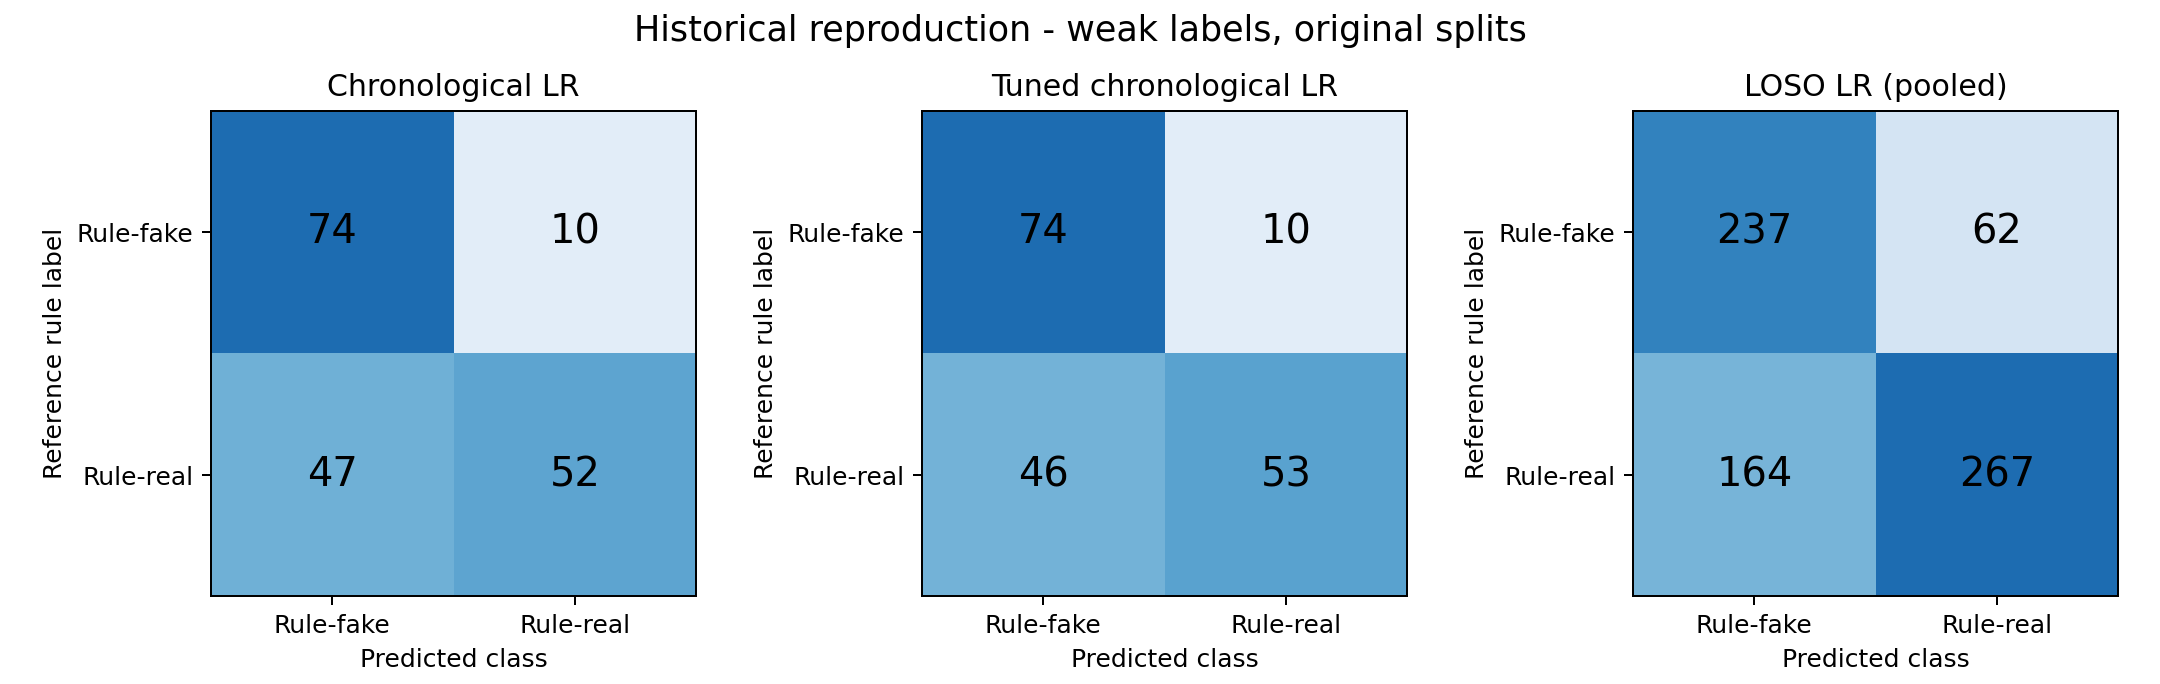
\includegraphics[width=\linewidth]{figures/confusion_matrices.png}
\caption{Reproduced historical confusion matrices. Class labels are generated by the original rules, and the partitions retain the limitations identified by WP01.}\label{fig:cms}\end{figure}
\begin{figure}[htbp]\centering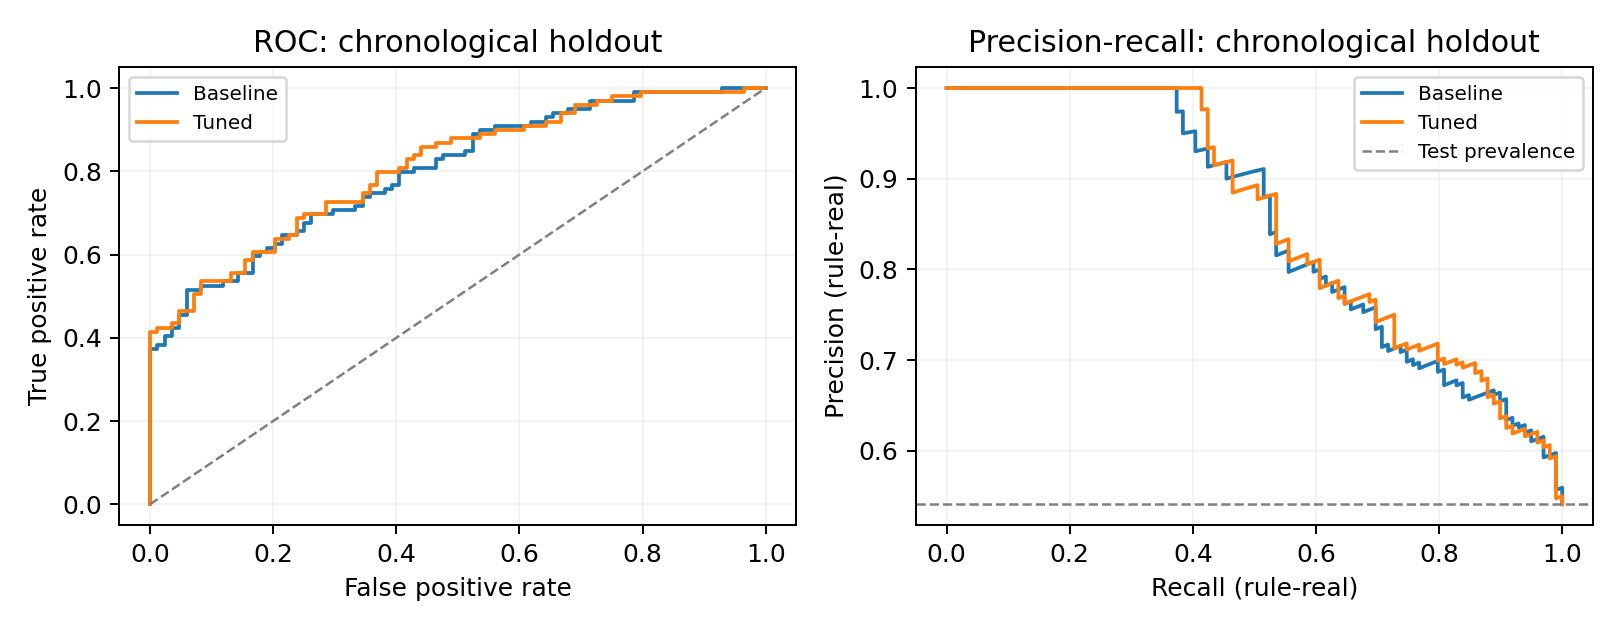
\includegraphics[width=\linewidth]{figures/roc_pr_curves.png}
\caption{Historical chronological ROC and precision--recall curves. These curves are evidence of reproduction, not corrected-validation performance.}\label{fig:rocpr}\end{figure}

\section{Integrity and methodological audit}
The audit reported no disagreement in the stored sharp-jump, sharp-drop, return-to-normal or suspected-fake calculations within the exported intermediates. No candidate-rule violations or event-duration count mismatches were found at this boundary. The absence of disagreements is useful, but only verifies internal agreement with the exported calculations; it cannot prove that the source sensor records or station metadata were correct. The earlier EDA notebook was inspected but was not fully rerun from raw data during WP01.

The audit identified three methodological risks requiring correction. First, training and testing observations shared the same outer-boundary timestamp. Second, two inner tuning folds shared a sensor event between fitting and validation. Third, completed-event summaries appeared for 89 labelled candidate-hour rows before those events had ended. Those summaries require a retrospective decision-time interpretation or different feature construction. A further fundamental issue is the circularity between heuristic labels and their predictors. For example, all historical rule-fake examples had one-hour candidate duration, and the model included duration as a feature. Good performance in this setting may reflect strong reproduction of the labelling logic rather than discovery of independent environmental truth.

\section{Corrected results: pending WP02}
\todo{Replace or supplement historical metrics with the verified corrected dataset counts, split protocol, Logistic Regression results and class-wise metrics returned by Work. Do not copy the historical scores into a table labelled ``corrected''. Document the selected decision time and event/group leakage checks.}
\todo{Insert the final temporal-only versus spatial-feature comparison on identical examples and partitions. Add RF, boosting, SVM and ablation results only if those experiments actually ran. Include error analysis, per-fold class support and new figure files from the project.}

\chapter{Discussion}
\section{What the reproduced findings do and do not demonstrate}
The reproducibility audit provides a meaningful starting point because the recorded model outputs were independently generated again from the exported candidate table. This reduces uncertainty about whether the archived notebook results were incidental artefacts of saved output cells. The exact reproduction of confusion matrices supports the correctness of the implementation at the archived boundary under the specified environment. However, a reliable computational calculation can still correspond to a weak scientific test. It is therefore necessary to separate the question ``Can the model reproduce these rule labels?'' from ``Can the model establish whether a pollution event was physically genuine?''

The historical classifier appears relatively selective when it predicts the rule-real category but misses many rule-real observations. The combination of relatively high precision and moderate recall shows why aggregate accuracy or AUC alone does not characterise the operational trade-off. For an alerting context, the relative cost of missing a credible episode and issuing a false alert must be considered. At the same time, because labels are heuristic, the false positives and false negatives in the available confusion matrix are disagreements with rules, not adjudicated environmental errors. Claims about public-health consequences should therefore be phrased as motivations, not measured outcomes of this experiment.

The weak-label problem is more serious than ordinary imbalance. If the reference itself is defined in part by event duration, concentration changes and neighbour agreement, a sufficiently flexible model can learn these same criteria. A perfect match with the labels would not necessarily be a perfect classifier of real pollution. Independent review is important because it provides an opportunity to identify cases where the rule's assumptions fail. Examples include genuine highly localised emissions, neighbouring sensors with missing data and prolonged high concentrations that do not continue to meet the sharp-rise detector. If reviewed cases remain few or ambiguous, the conclusion must acknowledge that limitation rather than asserting external validity.

\section{Interpretation of spatial evidence}
Spatial information is scientifically interesting because a distributed monitoring network can observe patterns unavailable to an isolated sensor. A common response at nearby devices may support a wider event, and the absence of agreement may motivate additional review. But geographic distance is only one aspect of shared exposure. Wind direction, landscape, building environments and local sources can cause spatial heterogeneity. Consequently, an IDW feature should be interpreted as a summary of available neighbour measurements, not a physical transport model. A robust experiment would compare spatial and temporal arms on identical held-out cases, with location metadata checked and missing-neighbour behaviour reported.

This comparison is also important for identifying whether the research adds evidence beyond a rule-based classifier. A richer model can achieve high agreement with rule labels merely by encoding their ingredients. One useful control is to compare models with and without event duration, spatial availability and rule-adjacent features. Another is to measure how conclusions change on independently reviewed cases rather than only on the weak-labelled training distribution. Such analyses can reveal whether apparent gains are sensitive to assumptions or reflect genuinely informative contextual features. They should be reported only after execution, and no benefit should be claimed in advance.

\section{Implications for future alerting}
Retrospective validation can be useful even if it cannot provide immediate warning at the first moment of a spike. It can support subsequent quality assurance, flag suspicious records, assist analysts in prioritising reviews and inform whether a recorded incident merits further investigation. The cost is delay: an event must finish and relevant follow-up information must arrive. The report should quantify this delay once the retrospective decision rule is fixed. A separate early-warning model would require a different set of features and a different evaluation design, not merely an earlier timestamp attached to the same completed-event summaries.

A deployed monitoring system would also have to handle unconfirmed candidates instead of ignoring them. The present supervised experiment excludes most uncertain cases. An operational workflow might explicitly defer a decision, request human review or present a confidence indication. It should not convert low neighbour coverage into evidence of sensor failure. Quality, location and missingness flags need consistent treatment, and predictions should be recorded with the data and model versions that produced them. These considerations are implementation implications supported by the project's failure-mode analysis, not claims that a production alert system has been delivered.

\chapter{Limitations and Research Integrity}
\section{Label validity and selection bias}
The strongest limitation is the absence of established physical-event ground truth for the strict target labels. The labels encode plausible rules but do not prove that each candidate was a real emission or a sensor artefact. Requiring specific spatial agreement for real labels also tends to disadvantage genuinely local pollution events. Similarly, a class of suspected one-hour artefacts may exclude more complicated sensor faults. The binary sample removes the uncertain majority of candidates and therefore differs systematically from the population that a deployed model would face. Reported precision and recall cannot simply be interpreted as the performance of a general air-quality alarm.

\section{Dependence, timing and spatial coverage}
Candidate hours from the same event are correlated. Sensors in a common region may also experience shared air-mass conditions. An evaluation that ignores these dependencies can overstate the effective amount of independent evidence. The chronological and LOSO designs provide complementary perspectives but neither automatically proves transfer to a new neighbourhood or a future deployment with altered hardware and quality characteristics. Explicit grouping and careful information-time rules reduce particular leakage risks, while independent spatial transfer or prospective studies would be needed for broader generalisation claims.

The availability and reliability of neighbour measurements also vary. Sensors can be absent, intermittently connected or incorrectly mapped to station coordinates. Missing-neighbour cases are not equivalent to negative evidence and should not be treated as rule-fake by default. Because the initial reproduction was performed from a derived export, it could not independently quantify the effects of upstream duplicates, station mapping or raw quality filters. WP02 is responsible for verifying these issues in the local project. Until then, this draft records them as unresolved checks rather than completed cleaning results.

\section{Reproducibility and ethical reporting}
Reproducibility is supported by retaining original notebooks, code versions, dataset identities, split files, model parameters, predictions and source manifests. The scientific report should trace each final table and figure to an executed artifact. Any statement that a model was trained, a test passed or a feature improved accuracy needs corresponding evidence. Claims should not be inflated by comparing metrics from incompatible evaluation protocols or reporting uncertain weak-label values as environmental ground truth.

The final capstone report must also meet the university's academic-integrity requirements. The official AI declaration belongs in the front matter and must honestly describe relevant AI assistance. The student must inspect and own the scientific conclusions, verify sources and be prepared to defend the methodology in discussion with the supervisor. An automated writing draft is a starting point for independent revision, not a substitute for the researcher's understanding. Turnitin checks and institutional approval decisions cannot be simulated by the report-generation process.

\chapter{Conclusion and Next Steps}
The historical SACAQM experiment demonstrates a reproducible pipeline for selecting unusual hourly \pmf{} observations and training a model to classify a subset of them according to temporal and spatially informed rules. From the exported candidate table, the earlier Logistic Regression results were recreated, including moderate rule-real recall and appreciable false negatives. The same audit also identified important limitations involving label circularity, validation partitions and the availability of completed-event information. These findings mean that the reproduced scores should be retained as historical baselines rather than presented as final proof of physical-event discrimination.

The immediate research priority is to complete WP02's raw-data verification, specify retrospective prediction time, validate event-safe partitions and rerun the reference model. A subsequent controlled comparison may assess whether spatial information contributes useful evidence beyond temporal features. The final interpretation should state exactly which experiment was performed and which form of generalisation it supports. The intended contribution is not merely a numerical score, but a transparent account of how candidate validation can be studied, reproduced and improved without overstating the evidence.

\todo{Rewrite the final two conclusion paragraphs when corrected WP02/model-comparison results are available. State measured contributions only, relate results explicitly to the central research question, and include concrete limitations and future work.}
\appendix
\chapter{Finalisation Checklist}
\begin{enumerate}
\item Confirm the official course-report title, student identity, supervisor name and submission date.
\item Insert the actual completed official postgraduate AI declaration as front matter (replace placeholder).
\item Verify the corrected WP02 dataset sizes, split IDs, metrics, feature definitions and plots against local code.
\item Use matched evaluation splits for comparisons and label historical scores unambiguously.
\item Verify every bibliographic entry against the publisher version; correct any provisional author fields.
\item Compile this LaTeX source with the supplied \texttt{references.bib} and inspect the PDF visually.
\item Check final word count at least 4,500 words, using the course's definition of countable material.
\item Run Turnitin generator 1/2 on the final PDF; review each individual source match. Do not assume compliance.
\item Ensure a brief report defence meeting with the supervisor has been scheduled, as required.
\item Submit through the specified Moodle submission page, not directly to the supervisor.
\end{enumerate}
\begin{thebibliography}{99}
\bibitem[World Health Organization(2021)]{who2021}
World Health Organization. (2021).
\emph{WHO global air quality guidelines: Particulate matter (PM2.5 and PM10), ozone, nitrogen dioxide, sulfur dioxide and carbon monoxide}.
World Health Organization. \url{https://www.who.int/publications/i/item/9789240034228}.

\bibitem[McKenzie et~al.(2024)]{mckenzie2024}
McKenzie, R. P., Cervello, A., Chabalala, V., et al. (2024).
A cost-effective air quality monitoring system for the Global South.
\emph{2024 IEEE International Humanitarian Technologies Conference}, 1--7.
\url{https://doi.org/10.1109/IHTC61819.2024.10855074}.

\bibitem[Huang et~al.(2022)]{huang2022}
Huang, J., et al. (2022).
Field evaluation and calibration of low-cost air pollution sensors for environmental exposure research.
\emph{Sensors}, 22(6), 2381.
\url{https://doi.org/10.3390/s22062381}.

\bibitem[Kapoor and Narayanan(2023)]{kapoor2023}
Kapoor, S. and Narayanan, A. (2023).
Leakage and the reproducibility crisis in machine-learning-based science.
\emph{Patterns}, 4(9), 100804.
\url{https://doi.org/10.1016/j.patter.2023.100804}.

\bibitem[Pedregosa et~al.(2011)]{pedregosa2011}
Pedregosa, F., et al. (2011).
Scikit-learn: Machine learning in Python.
\emph{Journal of Machine Learning Research}, 12, 2825--2830.
\url{https://www.jmlr.org/papers/v12/pedregosa11a.html}.

\bibitem[Breiman(2001)]{breiman2001}
Breiman, L. (2001). Random forests.
\emph{Machine Learning}, 45, 5--32.
\url{https://doi.org/10.1023/A:1010933404324}.

\bibitem[Friedman(2001)]{friedman2001}
Friedman, J. H. (2001). Greedy function approximation: A gradient boosting machine.
\emph{The Annals of Statistics}, 29(5), 1189--1232.
\url{https://doi.org/10.1214/aos/1013203451}.

\bibitem[Cortes and Vapnik(1995)]{cortes1995}
Cortes, C. and Vapnik, V. (1995). Support-vector networks.
\emph{Machine Learning}, 20, 273--297.
\url{https://doi.org/10.1007/BF00994018}.

\bibitem[Chabalala(2026)]{chabalala2026}
Chabalala, V. (2026). Spatiotemporal graph neural networks for PM2.5 concentration forecasting.
\emph{Air}, 4(1), 2.
\url{https://doi.org/10.3390/air4010002}.
\end{thebibliography}
\end{document}
